%------------------------------------------------
\section{Tổng quan}

%------------------------------------------------
\begin{frame}
\label{Maths}
	\frametitle{TỔNG QUAN TẤM PIN NĂNG LƯỢNG MẶT TRỜI}
	\begin{center}
		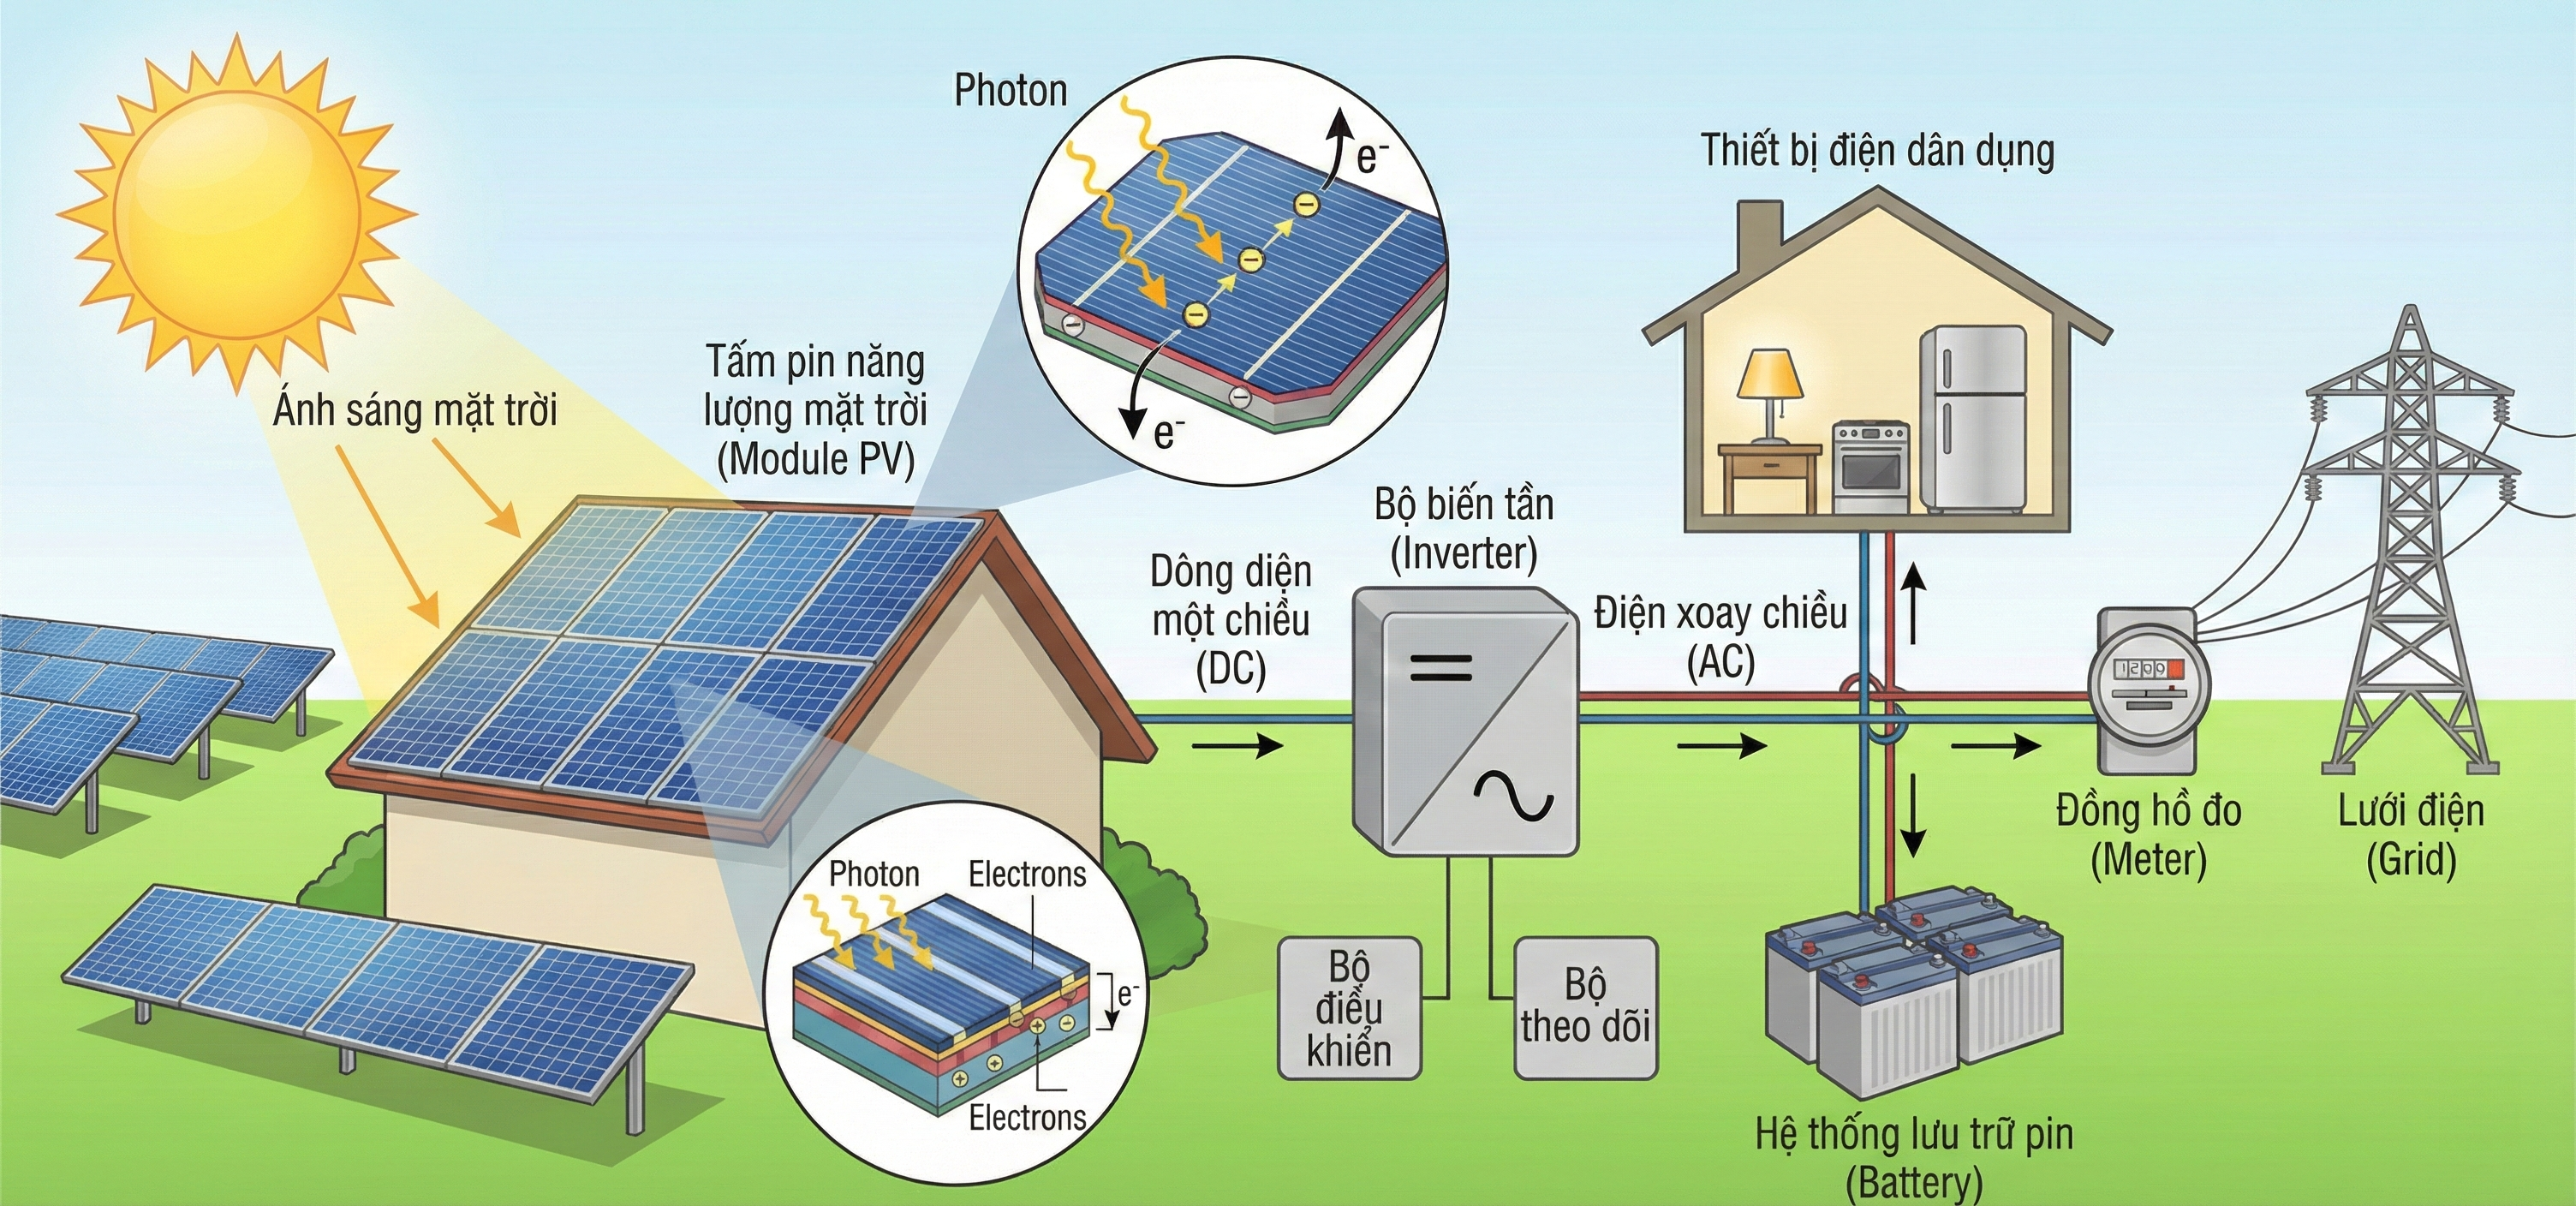
\includegraphics[width=0.8\textwidth]{images/TongQuan/pinmattroi.png}
	\end{center}
\end{frame}

%------------------------------------------------
\begin{frame}
	\frametitle{TÌNH HÌNH HỆ THỐNG PIN MẶT TRỜI TRÊN THẾ GIỚI}
	
	\vspace{0.3cm}
	
	\begin{columns}[t]
		% Cột 1: BÙNG NỔ
		\begin{column}{0.3\textwidth}
			\centering
			\includegraphics[width=0.5\textwidth]{images/TongQuan/icons/bungno.png}
			
			\vspace{0.3cm}
			
			{\Large\textbf{BÙNG NỔ}}
			
			\vspace{0.4cm}
			
			\small
			Diện mặt trời chiếm \\
			\textcolor{orange}{\textbf{73\%}} tổng công suất \\
			năng lượng tái tạo \\
			tăng thêm toàn cầu \\
			năm 2023.
		\end{column}

		\vrule width 1pt
		
		% Cột 2: CHI PHÍ
		\begin{column}{0.3\textwidth}
			\centering
			\includegraphics[width=0.5\textwidth]{images/TongQuan/icons/chiphi.png}
			
			\vspace{0.3cm}
			
			{\Large\textbf{CHI PHÍ}}
			
			\vspace{0.4cm}
			
			\small
			Chi phí lắp đặt đã giảm sâu \\
			\textcolor{orange}{\textbf{85\%}} sau một thập kỷ, trở \\
			thành nguồn năng lượng \\
			dễ tiếp cận nhất.
		\end{column}

		\vrule width 1pt
		
		% Cột 3: TIỀM NĂNG
		\begin{column}{0.3\textwidth}
			\centering
			\includegraphics[width=0.5\textwidth]{images/TongQuan/icons/tiemnang.png}
			
			\vspace{0.3cm}
			
			{\Large\textbf{TIỀM NĂNG}}
			
			\vspace{0.4cm}
			
			\small
			Việt Nam nằm trong \\
			``vùng đỏ'' bức xạ nhiệt, \\
			mang hữu tiềm năng tự \\
			nhiên lý tưởng để phát \\
			triển điện mặt trời.
		\end{column}
	\end{columns}
	
\end{frame}

\begin{frame}
\label{Bungno}
	\frametitle{TÌNH HÌNH HỆ THỐNG PIN MẶT TRỜI TRÊN THẾ GIỚI}
	\begin{center}
		\includegraphics[width=0.7\textwidth]{images/TongQuan/bieudobungno.png}
	\end{center}
\end{frame}

\begin{frame}
\label{Chiphi}
	\frametitle{TÌNH HÌNH HỆ THỐNG PIN MẶT TRỜI TRÊN THẾ GIỚI}
	\begin{center}
		\includegraphics[width=0.6\textwidth]{images/TongQuan/bieudochiphi.png}
	\end{center}
\end{frame}

\begin{frame}
\label{Nhiet}
	\frametitle{TÌNH HÌNH HỆ THỐNG PIN MẶT TRỜI TRÊN THẾ GIỚI}
	\begin{center}
		\includegraphics[width=0.8\textwidth]{images/TongQuan/bieudonhiet.png}
	\end{center}
\end{frame}

%------------------------------------------------
\section{Testing}

%------------------------------------------------
\begin{frame}
	\frametitle{Blocks}
    	\begin{block}{Block Title}
    		Block 1
    	\end{block}
    	
    	\begin{exampleblock}{Example Block Title}
    		Block 2
    	\end{exampleblock}
    	
    	\begin{alertblock}{Alert Block Title}
    		Block 3
    	\end{alertblock}
    	
    	\begin{block}{}
    		Block without a title
    	\end{block}
\end{frame}
